%license:BSD-3-Clause
%copyright-holders:Michele Maione
%============================================================
%
%	Piattaforma di cloud gaming per giochi arcade
%
%============================================================
\chapter{Tecnologie}

Lorem ipsum dolor sit amet, consectetur adipiscing elit, sed do eiusmod tempor incididunt ut labore et dolore magna aliqua. Ut enim ad minim veniam, quis nostrud exercitation ullamco laboris nisi ut aliquip ex ea commodo consequat. Duis aute irure dolor in reprehenderit in voluptate velit esse cillum dolore eu fugiat nulla pariatur. Excepteur sint occaecat cupidatat non proident, sunt in culpa qui officia deserunt mollit anim id est laborum.


\section{Proposed system}
Una caratteristica fondamentale del sistema è l'usabilità e per questo, lato client, il browser web è stata la scelta più ovvia.
Esistono alcune tecnologie di streaming per i browser web: WebSocket, HLS, DASH e WebRTC\cite{Audio_and_video_delivery}.

WebSocket è un protocollo di comunicazione che fornisce canali di comunicazione full-duplex su una singola connessione TCP, con una latenza inferiore rispetto a HLS e DASH.

HTTP Live Streaming (HLS) è il protocollo di streaming ad alta latenza più popolare su HTTP per video on demand (video preregistrato) sviluppato da Apple.

Dynamic Adaptive Streaming over HTTP (DASH) è una tecnica di streaming bit rate adattiva di Moving Picture Experts Group (MPEG), che consente lo streaming di alta qualità di contenuti multimediali su HTTP.

Web Real-Time Communication (WebRTC) è un progetto per la comunicazione in tempo reale basato sul protocollo SRTP (Secure Real-time Transport Protocol). Pertanto, per ottenere il flusso SRTP nel browser è necessario un server WebRTC\cite{High_Performance_Browser_Networking}.

\begin{figure}[H]
	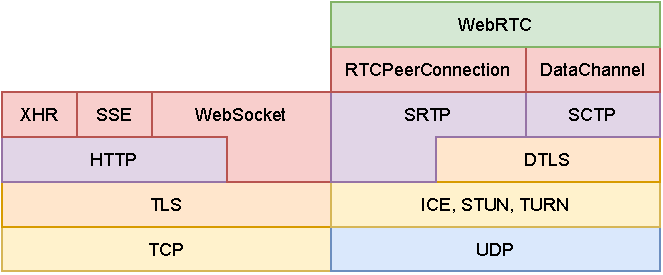
\includegraphics[width=\linewidth]{immagini/webprotocols}
	\caption{API, protocolli e servizi di rete del browser di alto livello}
	\label{fig:webprotocols}
\end{figure}

Questo progetto è pensato per essere utilizzato in stand di retro-gaming in eventi commerciali per l'industria IT e dei videogiochi, verrà eseguito su una rete locale e gli utenti sono connessi tramite WiFi, quindi la differenza di velocità tra TCP e UDP diventa trascurabile, quindi il la scelta è ricaduta su WebSocket perché è un protocollo di comunicazione standardizzato dal 2011, è pienamente supportato da tutti i browser moderni, è semplice e non richiede l'utilizzo di protocolli aggiuntivi o configurazioni complesse a differenza di WebRTC.

\begin{figure}[H]
	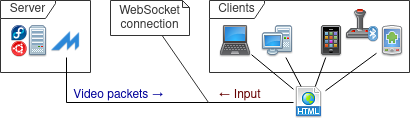
\includegraphics[width=\linewidth]{immagini/proposed_system}
	\caption{Panoramica del sistema}
	\label{fig:proposed_system}
\end{figure}

Il sistema è costituito da un server di gioco, che può essere Linux, Windows o macOS, che esegue MAME e una pagina HTML5 che funge da front-end.

Il programma sta ascoltando una connessione WebSocket che include parametri, come il nome del gioco. Una volta stabilita la connessione, il server invia informazioni sulla dimensione e le proporzioni del video e avvia il gioco. Il rendering e il missaggio audio del gioco vengono generati tramite SDL\footnote{SDL: Simple DirectMedia Layer, una libreria di sviluppo software multipiattaforma progettata per fornire un livello di astrazione hardware per componenti hardware multimediali del computer.}, Codificati e pacchettizzati in MPEG-TS\footnote{MPEG-TS: MPEG transport stream, è un formato contenitore digitale standard per la trasmissione e l'archiviazione di audio e video.} tramite FFmpeg\footnote{FFmpeg è una vasta suite open source di librerie e programmi per la gestione di video, audio, e altri file multimediali e stream.}. I pacchetti vengono inviati tramite WebSocket al client.

Lato client vari script si occuperanno di decodificare i dati audio / video ricevuti, catturare e inviare l'input dell'utente, sia dalla tastiera che dal gamepad, al server tramite WebSocket.

\section{MPEG}
Lorem ipsum dolor sit amet, consectetur adipiscing elit, sed do eiusmod tempor incididunt ut labore et dolore magna aliqua. Ut enim ad minim veniam, quis nostrud exercitation ullamco laboris nisi ut aliquip ex ea commodo consequat. Duis aute irure dolor in reprehenderit in voluptate velit esse cillum dolore eu fugiat nulla pariatur. Excepteur sint occaecat cupidatat non proident, sunt in culpa qui officia deserunt mollit anim id est laborum.

\subsection{Compression}
Lorem ipsum dolor sit amet, consectetur adipiscing elit, sed do eiusmod tempor incididunt ut labore et dolore magna aliqua. Ut enim ad minim veniam, quis nostrud exercitation ullamco laboris nisi ut aliquip ex ea commodo consequat. Duis aute irure dolor in reprehenderit in voluptate velit esse cillum dolore eu fugiat nulla pariatur. Excepteur sint occaecat cupidatat non proident, sunt in culpa qui officia deserunt mollit anim id est laborum.

\subsection{Video}
Lorem ipsum dolor sit amet, consectetur adipiscing elit, sed do eiusmod tempor incididunt ut labore et dolore magna aliqua. Ut enim ad minim veniam, quis nostrud exercitation ullamco laboris nisi ut aliquip ex ea commodo consequat. Duis aute irure dolor in reprehenderit in voluptate velit esse cillum dolore eu fugiat nulla pariatur. Excepteur sint occaecat cupidatat non proident, sunt in culpa qui officia deserunt mollit anim id est laborum.

\subsection{Audio}
Lorem ipsum dolor sit amet, consectetur adipiscing elit, sed do eiusmod tempor incididunt ut labore et dolore magna aliqua. Ut enim ad minim veniam, quis nostrud exercitation ullamco laboris nisi ut aliquip ex ea commodo consequat. Duis aute irure dolor in reprehenderit in voluptate velit esse cillum dolore eu fugiat nulla pariatur. Excepteur sint occaecat cupidatat non proident, sunt in culpa qui officia deserunt mollit anim id est laborum.

\subsection{Trasmission}
Lorem ipsum dolor sit amet, consectetur adipiscing elit, sed do eiusmod tempor incididunt ut labore et dolore magna aliqua. Ut enim ad minim veniam, quis nostrud exercitation ullamco laboris nisi ut aliquip ex ea commodo consequat. Duis aute irure dolor in reprehenderit in voluptate velit esse cillum dolore eu fugiat nulla pariatur. Excepteur sint occaecat cupidatat non proident, sunt in culpa qui officia deserunt mollit anim id est laborum.



\section{FFmpeg}
Lorem ipsum dolor sit amet, consectetur adipiscing elit, sed do eiusmod tempor incididunt ut labore et dolore magna aliqua. Ut enim ad minim veniam, quis nostrud exercitation ullamco laboris nisi ut aliquip ex ea commodo consequat. Duis aute irure dolor in reprehenderit in voluptate velit esse cillum dolore eu fugiat nulla pariatur. Excepteur sint occaecat cupidatat non proident, sunt in culpa qui officia deserunt mollit anim id est laborum\cite{FFmpeg_Documentation}.

\subsection{Libs.}
Lorem ipsum dolor sit amet, consectetur adipiscing elit, sed do eiusmod tempor incididunt ut labore et dolore magna aliqua. Ut enim ad minim veniam, quis nostrud exercitation ullamco laboris nisi ut aliquip ex ea commodo consequat. Duis aute irure dolor in reprehenderit in voluptate velit esse cillum dolore eu fugiat nulla pariatur. Excepteur sint occaecat cupidatat non proident, sunt in culpa qui officia deserunt mollit anim id est laborum.



\section{Simple DirectMedia Layer (SDL)}
SDL is a library that provides low level access to audio, keyboard, mouse, gamepad, 3D hardware, and 2D framebuffer across multiple platforms, also mobile. SDL it is built on top of the video display APIs of the O.S., a 3D rendering library and a library that interface to sound card\cite{SDL_Wiki}.

\begin{figure}[H]
	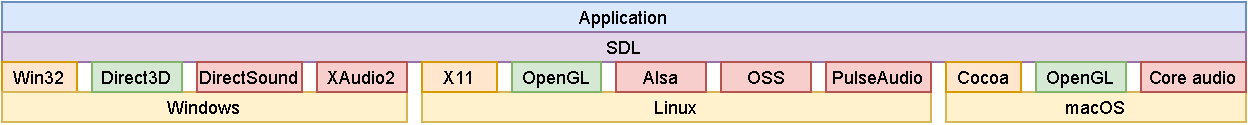
\includegraphics[width=\linewidth]{immagini/sdl}
	\caption{Abstraction layers of several SDL platforms}
	\label{fig:sdl}
\end{figure}

\subsection{Video}
The MAME is able to emulate 3D games but since a physical monitor is being emulated, what is sent to the various graphics libraries is a set of primitives and textures to be drawn, and for this reason the drawing is always carried out in 2D.

\begin{figure}[H]
	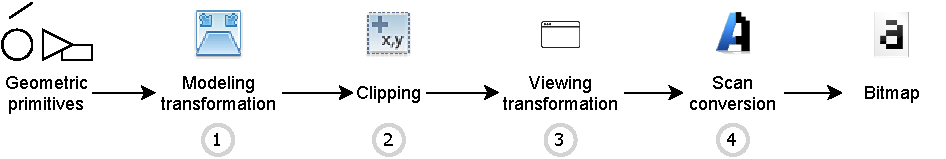
\includegraphics[width=\linewidth]{immagini/rendering_pipeline}
	\caption{2D rendering pipeline}
	\label{fig:rendering_pipeline}
\end{figure}

When the window is initialized an SDL 2D rendering context for the window is created through the function \textit{CreateRenderer}. For each emulated machine frame there is a draw phase using \textit{SetRenderDrawColor}, \textit{RenderFillRect} and \textit{RenderDrawLine}. In the end the function \textit{RenderPresent} is used to show the frame on the window.

In section \ref{SDL_renderer} other functions, used to modify this standard behaviour descripted above, are introduced.


\subsection{Audio}
Lorem ipsum dolor sit amet, consectetur adipiscing elit, sed do eiusmod tempor incididunt ut labore et dolore magna aliqua. Ut enim ad minim veniam, quis nostrud exercitation ullamco laboris nisi ut aliquip ex ea commodo consequat. Duis aute irure dolor in reprehenderit in voluptate velit esse cillum dolore eu fugiat nulla pariatur. Excepteur sint occaecat cupidatat non proident, sunt in culpa qui officia deserunt mollit anim id est laborum.



\section{Web APIs}
Web APIs are a set of APIs and interfaces that comprise the Web's powerful scriptability. Following those used in this project\cite{Web_APIs}.

\subsection{WebSocket}
WebSocket is a computer communications protocol providing full-duplex communication channels over a single TCP connection. It is compatible with HTTP because the WebSocket handshake uses the HTTP upgrade header to switch from the HTTP to the WebSocket protocol. It is natively supported by all browsers and its use is similar to normal sockets on both client and server sides. For these reasons it is the most used generic communication protocol on the web\cite{WebSocket_Web_APIs}.

\subsection{Canvas API}
The Canvas API provides a means for drawing graphics via JavaScript, is largely focuses on 2D graphics but when used by WebGL API can draws hardware-accelerated 2D and 3D graphics. It is fully supported by all browsers\cite{Canvas_API}.

\subsection{WebGL API}
WebGL is a JavaScript API, designed and maintained by the non-profit Khronos Group, for rendering interactive 2D and 3D graphics allowing GPU-accelerated usage of physics and image processing and effects. WebGL 1.0 is supported on all browsers, while WebGL 2.0 is being tested on Safari\cite{WebGL}.



\section{JavaScript libraries}
For the front-end, opensource JavaScript libraries were used for the input management and for decoding the movie.

\subsection{JSMpeg}
JSMpeg is a JavaScript library that consists of an MPEG-TS demuxer, MPEG1 video and MP2 audio decoders, WebGL and Canvas2D renderers and WebAudio sound output. JSMpeg can load static videos via Ajax and allows low latency streaming ($\sim$50ms) via WebSockets, it is released under the MIT License\cite{JSMpeg}.

\subsection{Keypress}
Keypress is a keyboard input capturing JavaScript utility focused on input for games, released under the Apache License 2.0. It is used to handle keyboard input in the front-end\cite{Keypress}.

\subsection{GameController.js}
GameController.js is a library that uses JavaScript and the standard Gamepad API, it is released under the MIT License. In the front-end it is used to manage gamepads, to allow couch multiplayer\cite{gameController_js}.